
\addtocontents{toc}{\vspace{\baselineskip}APPENDICES}
\setcounter{table}{0}
\renewcommand{\thetable}{\Alph{chapter}\arabic{table}}
\GrizzAppendix{Tables and Figures} \label{ch:extra}



\begin{figure}
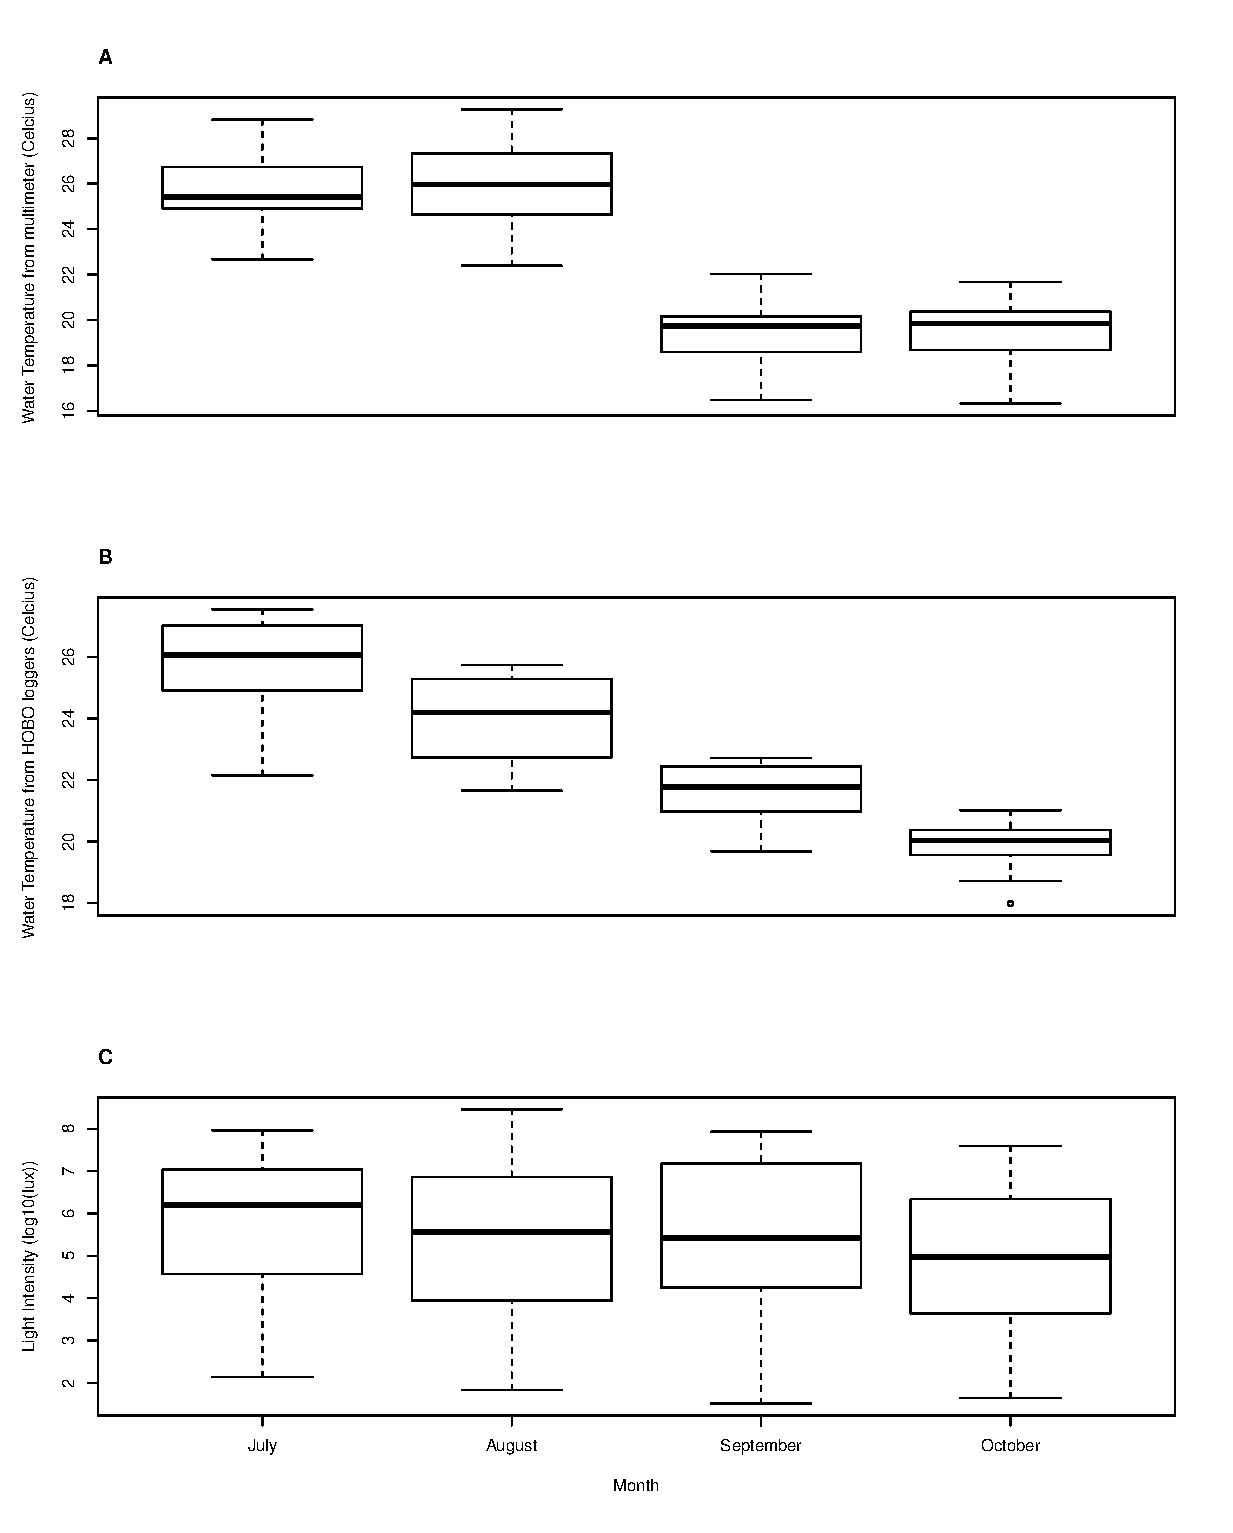
\includegraphics[width=\textwidth]{figures/hobo}
\caption{
(A): Boxplot summary of the average lake temperature measured at the time of sampling with hand-held multimeter 
(B): Boxplot summary of average lake temprature from HOBO loggers. 
(C): Boxplot summary of light intensity also measured by HOBO loggers.
} 
\label{fig:hobo}
\end{figure}


\begin{figure}[!h]
 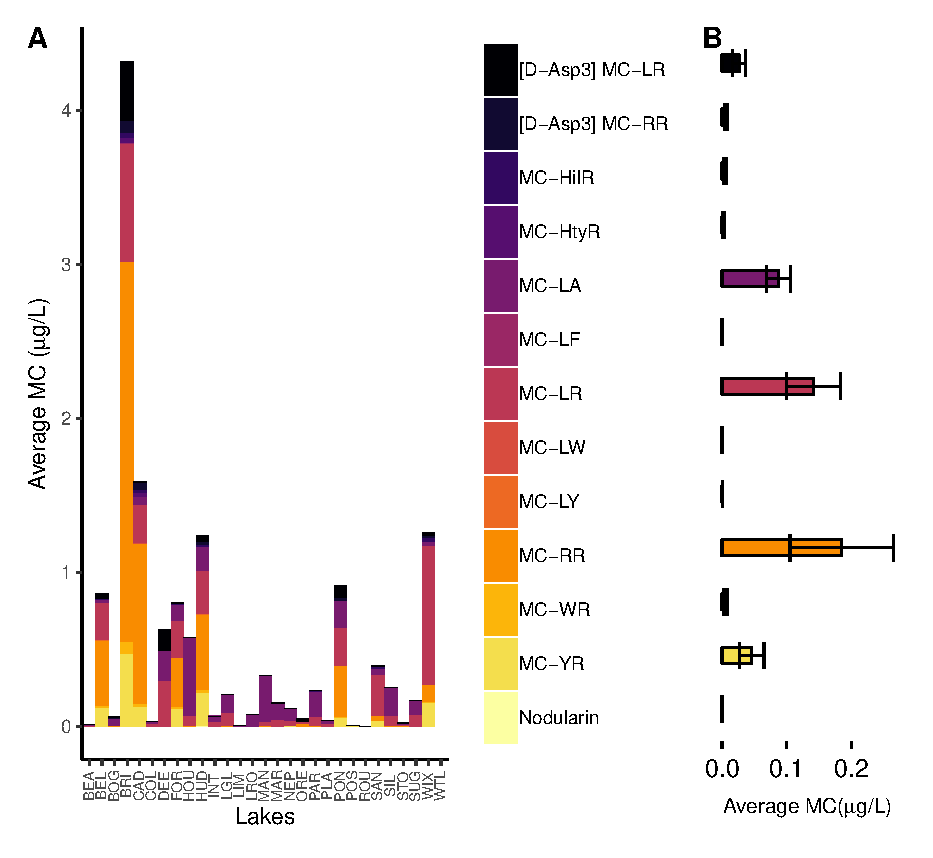
\includegraphics[width=\textwidth]{figures/congenerbar}
 \caption{
 (A): Average MC found at each lake in all four months. The height of each bar represents the total average of MC. The proportion of each congener is represented by color in each bar  
(B): Average MC congener with the included error bars represents one standard deviation of the mean}
 \label{fig:congenerbar}
\end{figure}



\begin{figure}[!ht]
\scalebox{1.14}{
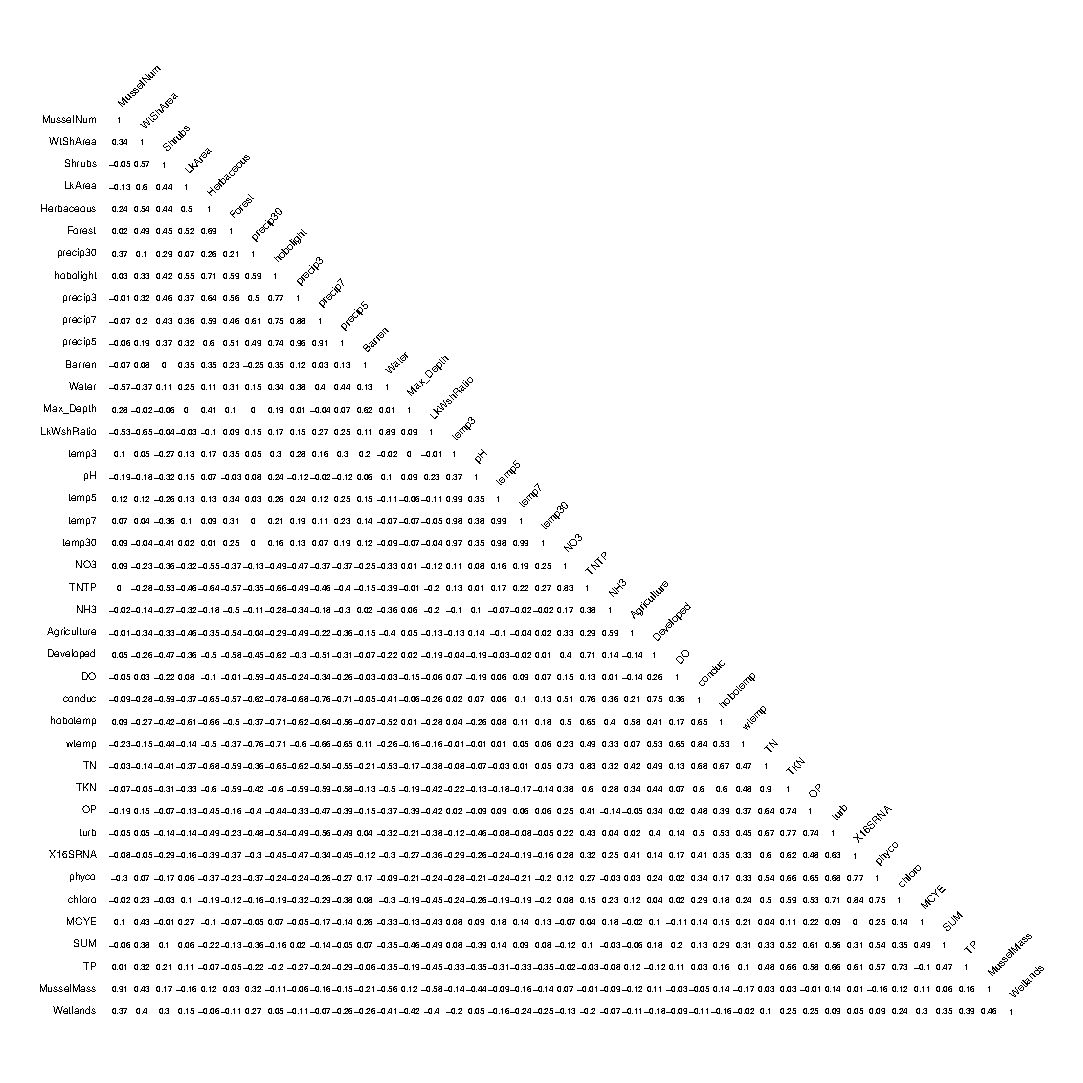
\includegraphics[width=\textwidth]{figures/matrixfull}}
\caption{Correlation matrix displaying Pearson's coefficient on the full data.}
\label{fig:matrixfull}
\end{figure}


\begin{figure}[!hp]
\centering
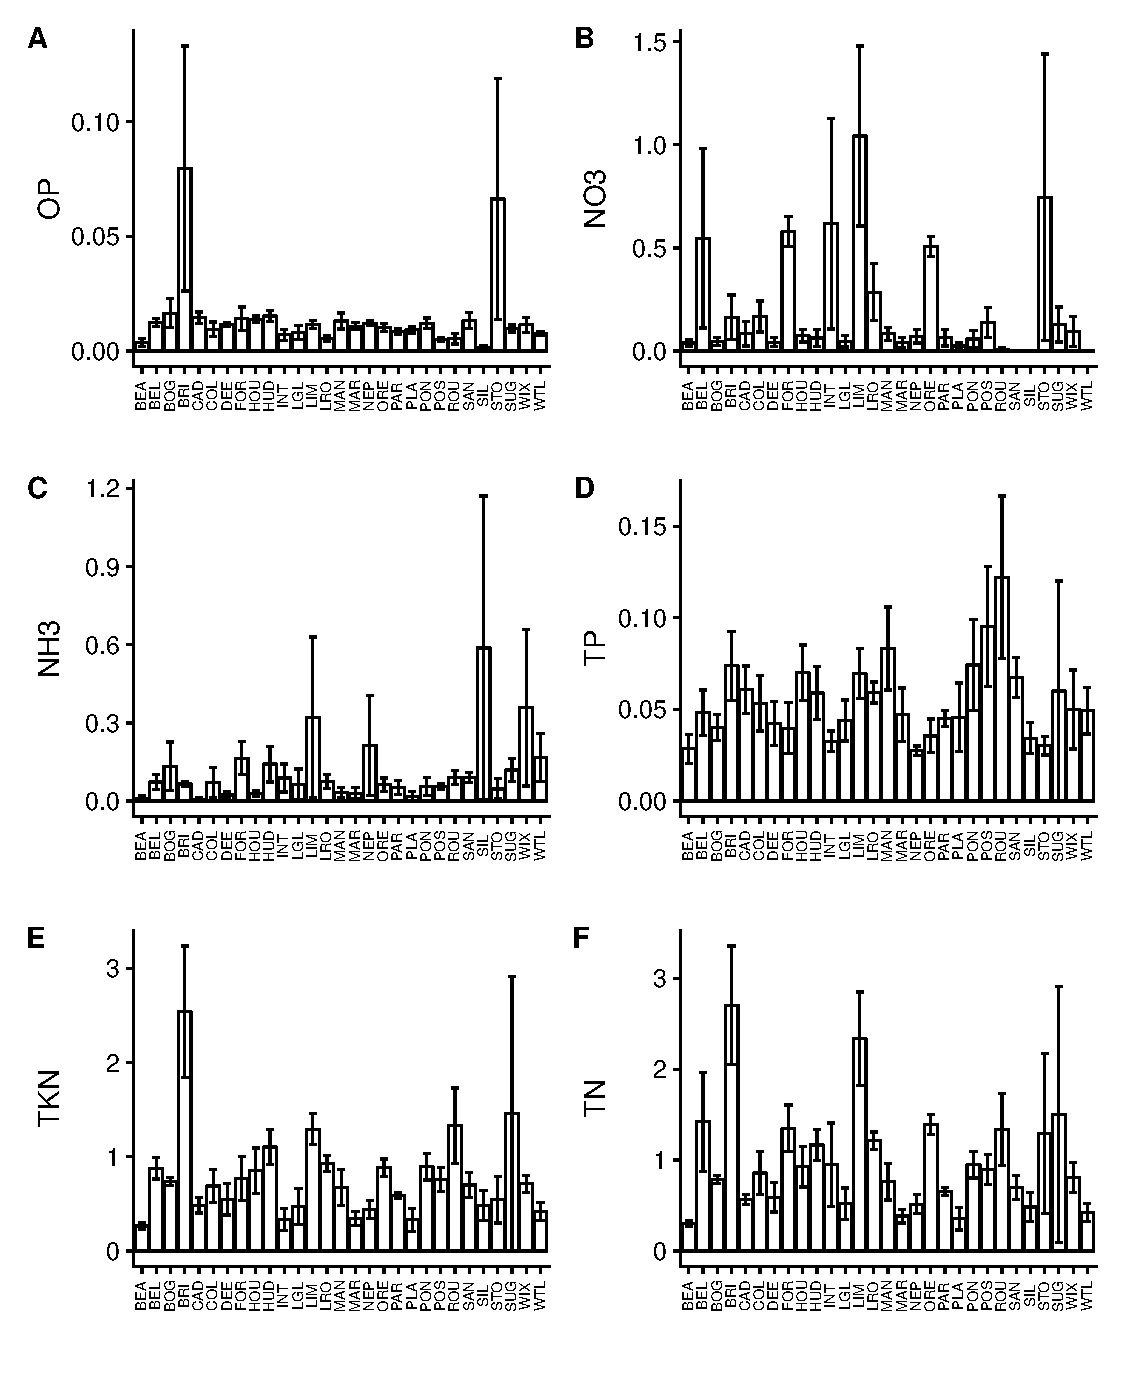
\includegraphics[width=\textwidth]{figures/nutboxplotlake}
\caption{Average nutrient concentrations for each lake for all of summer 2017. Figure (A): Orthophosphate (mg-P/L). Figure (B): Nitrate+nitrite (mg-N/L). Figure (C): Ammonia (mg-N/L). Figure (D): Total phosphorus (mg-P/L). Figure (E): Total Kjeldahl nitrogen (mg-N/L). Error bars represents one standard deviation of the mean. }
\label{fig:nutrients}
\end{figure}


\begin{figure}[!hp]
\centering
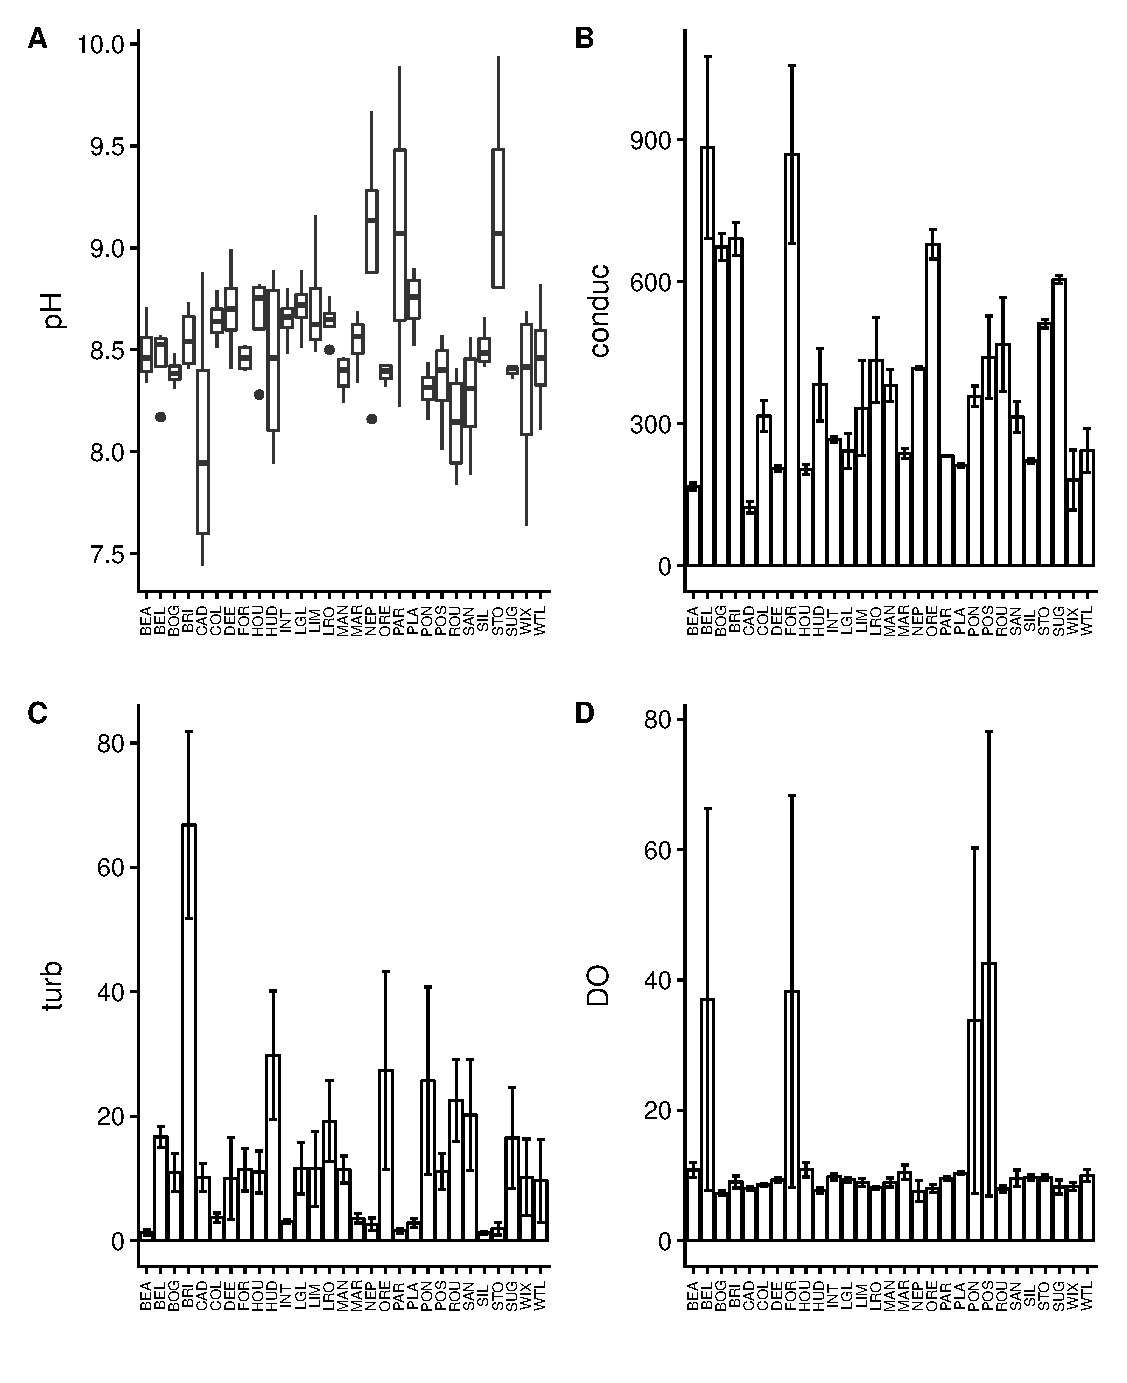
\includegraphics[width=\textwidth]{figures/watboxplotlake.eps}
\caption{Summary of measured water chemical parameters. Figure (A): A box and whisker plot of pH. Figure (B): Bar plots of average conductance. Figure (C): Average turbidity. Figure(D): Average dissolved oxygen. }
  \end{figure}
